\documentclass[a4paper, 10pt]{article}
\title{ECE253---Digital Systems}
\author{Jonah Chen}

\usepackage[utf8]{inputenc}
\usepackage[ma rgin=0.5in]{geometry}

\usepackage{braket}
\usepackage{physoly}
\usepackage{currfile}
\usepackage{gensymb}
\usepackage{amssymb}
\usepackage{pgf,tikz,pgfplots}
\usepackage{mathrsfs}
\usepackage{textcomp}
\usepackage{circuitikz}
\usetikzlibrary{arrows}
\numberwithin{equation}{section}
\pgfplotsset{compat=1.16}
\begin{document}
\sffamily
\maketitle
\tableofcontents

\section{Number Conversions}

\begin{itemize}
    \item Computers use binary. We use hexadecimal to make it less error-prone writing binary numbers.
    \item Convert binary to hex: grouping four bits together makes the conversion easier. $0101\:1110=5e$.
    \item Converting hex to binary: $a6=1010\:0110$
    \item Converting binary to decimal: find the bit positions for all the ``1''s. $101\:0111=2^6+2^4+2^2+2^1+2^0=87$.
    \item Converting decimal to binary: Repeatedly divide by two and get quotient and remainder. The remainders from the binary digits from least significant to most significant bits.
    \begin{align*}
        76/2&=38\\
        38/2&=19\\
        19/2&=9+1/2\\
        9/2&=4+1/2\\
        4/2&=2\\
        2/2&=1\\
        1/2&=0+1/2\\
    \end{align*}
    Thus, $76=1001100$. 
    % 1000
    % 256000=256*1000
    % 256144=256000+144
    \item Converting hex to decimal: $3e=3\times 16+14=62$.
    \item Converting decimal to hex: We can use algorithmic way, which is repeatedly dividing by sixteen and take the remainders to extract the hex digits but dividing by 16 is very difficult. So, first convert to binary then convert to hex. $96=110\:0000=60$
\end{itemize}

\section{Binary addition}
\begin{itemize}
    \item Each step of computation has three inputs and two outputs. 
\end{itemize}

\section{Primative logic gates}
\begin{center}
    \begin{tabular}{|c c|c|c|c|c|}
        $x$ & $y$ & $x+y$ & $xy$ & $\overline{x}$ & $\overline{y}$\\
        \hline
        0 & 0 & 0 & 0 & 1 & 1\\
        0 & 1 & 1 & 0 & 1 & 0\\
        1 & 0 & 1 & 0 & 0 & 1\\
        1 & 1 & 1 & 1 & 0 & 0
    \end{tabular}
\end{center}
\begin{tikzpicture}
    \begin{circuitikz}
        \node[npn]{};
    \end{circuitikz}
\end{tikzpicture}

\begin{example}
    Say $X$ is a 3-bit number, with bits $x_2x_1x_0$. Design a circuit with $X$ as input and one output $f$. $f$ should be 1 if $X\geq 5$, otherwise $f$ should be 0.

    \begin{center}
        \begin{tabular}{c|c c c|c}
            & $x_2$ & $x_1$ & $x_0$ & $f$\\
            \hline
            0 & 0 & 0 & 0 & 0\\
            1 & 0 & 0 & 1 & 0\\
            2 & 0 & 1 & 0 & 0\\
            3 & 0 & 1 & 1 & 0\\
            4 & 1 & 0 & 0 & 0\\
            5 & 1 & 0 & 1 & 1\\
            6 & 1 & 1 & 0 & 1\\
            7 & 1 & 1 & 1 & 1
        \end{tabular}
    \end{center}

    $f=x_2(x_1+x_0)$
    
\end{example}

\begin{itemize}
    \item Equation
    \item 
    \item Timing Diagram
\end{itemize}

\section{Boolean Algebra}
\begin{definition}
    \begin{itemize}
        \item A literal is a variable or not a variable
        \item A product term is a term that contains the ``and'' of literals
        \item A minterm is a product term that contains all the literals. Because there is a minimum set of input combinations (exactly 1 row of truth table) that cause the minterm to be true.
        \item A maxterm is a sum term that contains all the literals. Because there is a maximum set of input combinations (all but 1 truth table) that cause the maxterm to be true.
    \end{itemize}
\end{definition}
\begin{center}
    \begin{tabular}{|c c c|c|c|c|c|}
        $x_2$ & $x_1$ & $x_0$ & minterm & label & maxterm & label\\
        \hline
        0 & 0 & 0 & $\overline{x_2}\overline{x_1}\overline{x_0}$ & $m_0$ & $x_2+x_1+x_0$ & $M_0$\\
        0 & 0 & 1 & $\overline{x_2}\overline{x_1}{x_0}$ & $m_1$ & $x_2+x_1+\overline{x_0}$ & $M_1$\\
        0 & 1 & 0 \\
        0 & 1 & 1 \\
        1 & 0 & 0 \\ 
        1 & 0 & 1 \\
        1 & 1 & 0 & $x_2x_1\overline{x_0}$ & $m_6$ & $\overline{x_2}+\overline{x_1}+x_0$ & $M_6$\\
        1 & 1 & 1 & $x_2x_1x_0$ & $m_7$ & $\overline{x_2}+\overline{x_1}+\overline{x_0}$ & $M_7$
    \end{tabular}
\end{center}
\begin{example}
    \begin{center}
        \begin{tabular}{|c c c|c|c|}
            $x_2$ & $x_1$ & $x_0$ & $f$ & label\\
            \hline
            0 & 0 & 0 & 0 & $m_0$\\
            0 & 0 & 1 & 0 & $m_1$\\
            0 & 1 & 0 & 1 & $m_2$\\
            0 & 1 & 1 & 1 & $m_3$\\
            1 & 0 & 0 & 1 & $m_4$\\
            1 & 0 & 1 & 0 & $m_5$\\
            1 & 1 & 0 & 1 & $m_6$\\
            1 & 1 & 1 & 1 & $m_7$\\
        \end{tabular}
    \end{center}

    Canonical SOP form: 
    \begin{align}
        f&=\sum m(2,3,5,6,7)\\
        &=\overline{x_2}x_1\overline{x_0}+\overline{x_2}x_1x_0+x_2\overline{x_1}\overline{x_0}+x_2x_1\overline{x_0}+x_2x_1x_0\\
        &=\overline{x_2}x_1(\overline{x_0}+x_0)+x_2x_1(\overline{x_0}+x_0)+x_2\overline{x_1}\overline{x_0}\\
        &=\overline{x_2}x_1+x_2x_1+x_2\overline{x_1}\overline{x_0}\\
        &=x_1+x_2\overline{x_1}\overline{x_0}\\
        &=x_1+x_2\overline{x_0}
    \end{align}

    Canonical POS form:
    \begin{align}
        f&=\prod M(0,1,5)\\
        &=(x_2+x_1+x_0)(x_2+x_1+\overline{x_0})(\overline{x_2}+x_1+\overline{x_0})
    \end{align}

\end{example}
\begin{proposition}
    \begin{equation}
        a+bc=(a+b)(a+c)
    \end{equation}
    \begin{proof}
        \begin{align}
            (a+b)(a+c) &= a+ab+ac+bc\\
            &= a(1+b) + a(1+c) + bc\\
            &= a+bc
        \end{align}
    \end{proof}
\end{proposition}
\begin{proposition}[De-Morgan's Law]
    \begin{align}
        \overline{ab}&=\overline{a} + \overline{b}\\
        \overline{(a+b)}&=\overline{a}\overline{b}
    \end{align}
    Note this law is the means of translation between ``and'' and ``or''.
\end{proposition}
\begin{example}
    Gumball Factory: three sensors \begin{itemize}
        \item $s_2$: ball too large
        \item $s_1$: ball too small
        \item $s_0$: ball too light
    \end{itemize}
    \begin{center}
        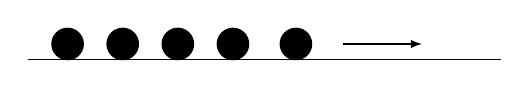
\begin{tikzpicture}
            \draw (0,0) -- (6,0);

            \draw[fill] (0.5,0.2) circle (0.2);
            \draw[fill] (1.2,0.2) circle (0.2);
            \draw[fill] (1.9,0.2) circle (0.2);
            \draw[fill] (2.6,0.2) circle (0.2);
            \draw[fill] (3.4,0.2) circle (0.2);
            \draw[-latex] (4,0.2) -- (5,0.2);
        \end{tikzpicture}
    \end{center}
    Design logic circuit with output one if ball is too large or it's too small and too light.
\end{example}

\begin{theorem}[Consensus]
    \begin{equation}
        xy+\overline{x}z+yz=xy+\overline{x}z
    \end{equation}
    \begin{proof}
        Use the property $1f=f$, $a+\overline{a}=1$.
        \begin{align}
            xy+\overline{x}z+yz=xy+\overline{x}z&=xy+\overline{x}z+(x+\overline{x})yz\\
            &=xy+xyz+\overline{x}z+\overline{x}yz\\
            &=xy+x\overline{z}
        \end{align}
    \end{proof}
\end{theorem}

\begin{example}
    \begin{align}
        f&=\overline a b+\overline a c+\overline b c\\
        &=\overline ab+\overline ac(b+\overline b)+\overline bc\\
        &=\overline ab+\overline acb+\overline ac\overline b+\overline bc\\
        &=\overline ab(1+c)+\overline bc(\overline a+1)\\
        &=\overline ab+\overline bc
    \end{align}
\end{example}
\subsection{Karnaugh maps}

\section{Multiplexers}
\begin{itemize}
    \item Recall 2-to-1 multiplexer $f=a\overline s+bs$.
    \item 4-to-1 multiplexer can be constructed with three 2-to-1 multiplexer. 
\end{itemize}
\end{document}
